\begin{figure}[htbp]\centering
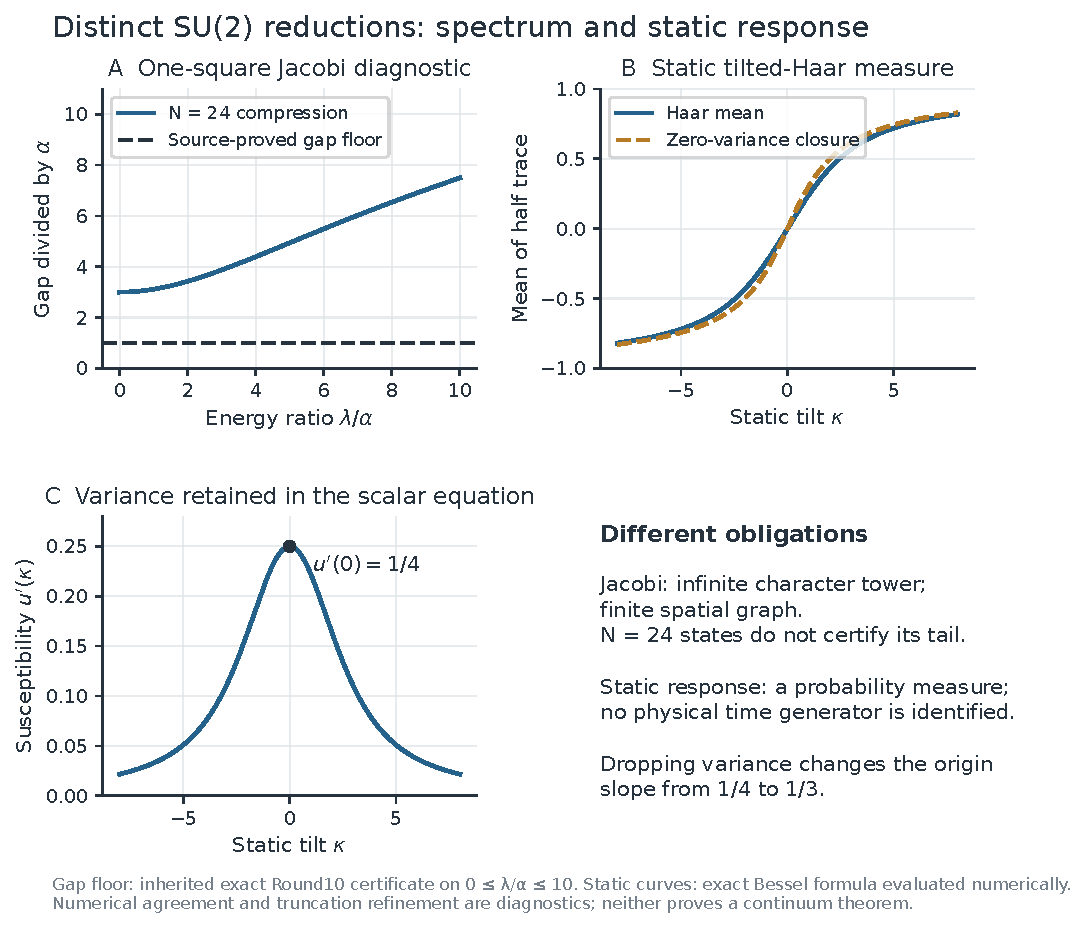
\includegraphics[width=\textwidth]{figures/jacobi_static.pdf}
\caption{Two distinct benchmarks. The one-square Jacobi eigenvalue curves are finite-matrix numerical diagnostics; the recorded continuous full-space certificate has its own tail and interval proof. The tilted-Haar mean and variance are static quantities, not a physical trajectory. Plot data and parameters are supplied with the calculators.}
\label{fig:jacobi-static}
\end{figure}

\begin{figure}[htbp]\centering
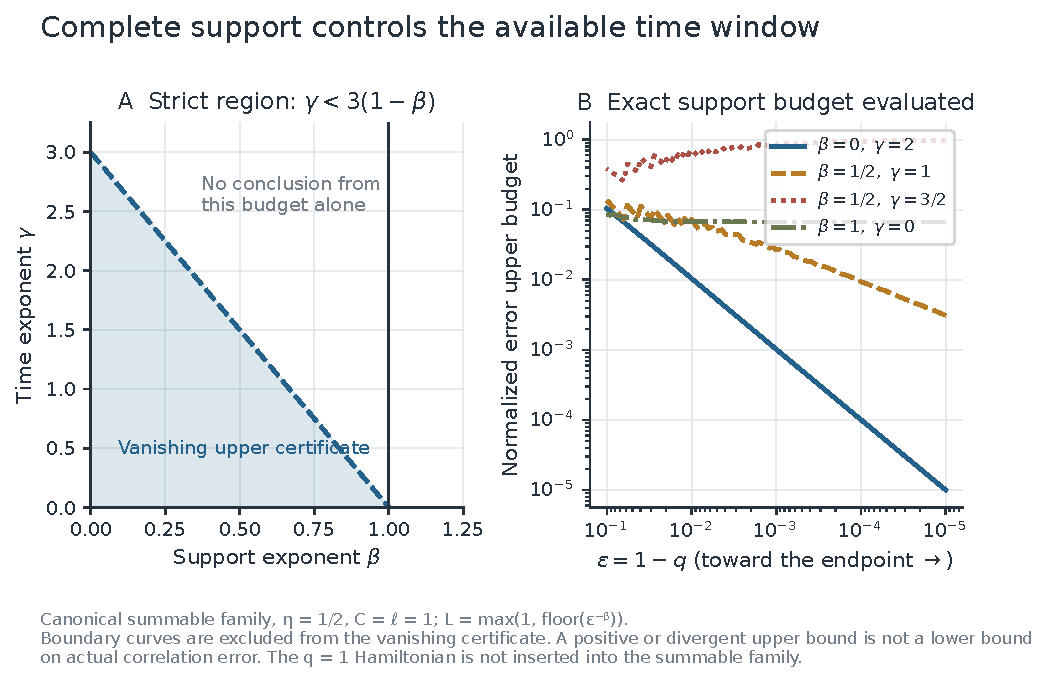
\includegraphics[width=\textwidth]{figures/support_window.pdf}
\caption{Sufficient support/time windows and evaluated upper budgets. The strict exponent region follows from the stated complete-support asymptotics. Values outside it indicate failure of this sufficient certificate, not proof that the actual correlation error diverges.}
\label{fig:support-window}
\end{figure}

\begin{figure}[htbp]\centering
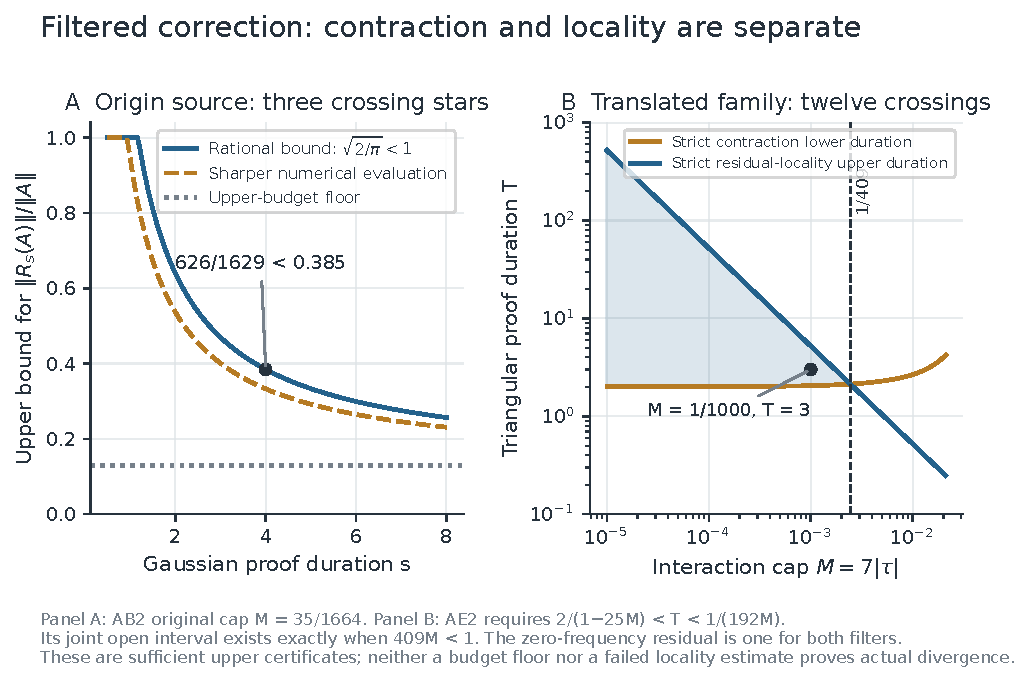
\includegraphics[width=\textwidth]{figures/filter_budgets.pdf}
\caption{Full-source Gaussian contraction and compact-filter certificate compatibility. Gaussian duration is a proof regulator. The compact construction has a smaller admitted coupling range and counts all translated crossings. The original-cap incompatibility concerns these sufficient bounds, not every possible filter or a lower bound on an actual error.}
\label{fig:filter-budgets}
\end{figure}

\begin{figure}[htbp]\centering
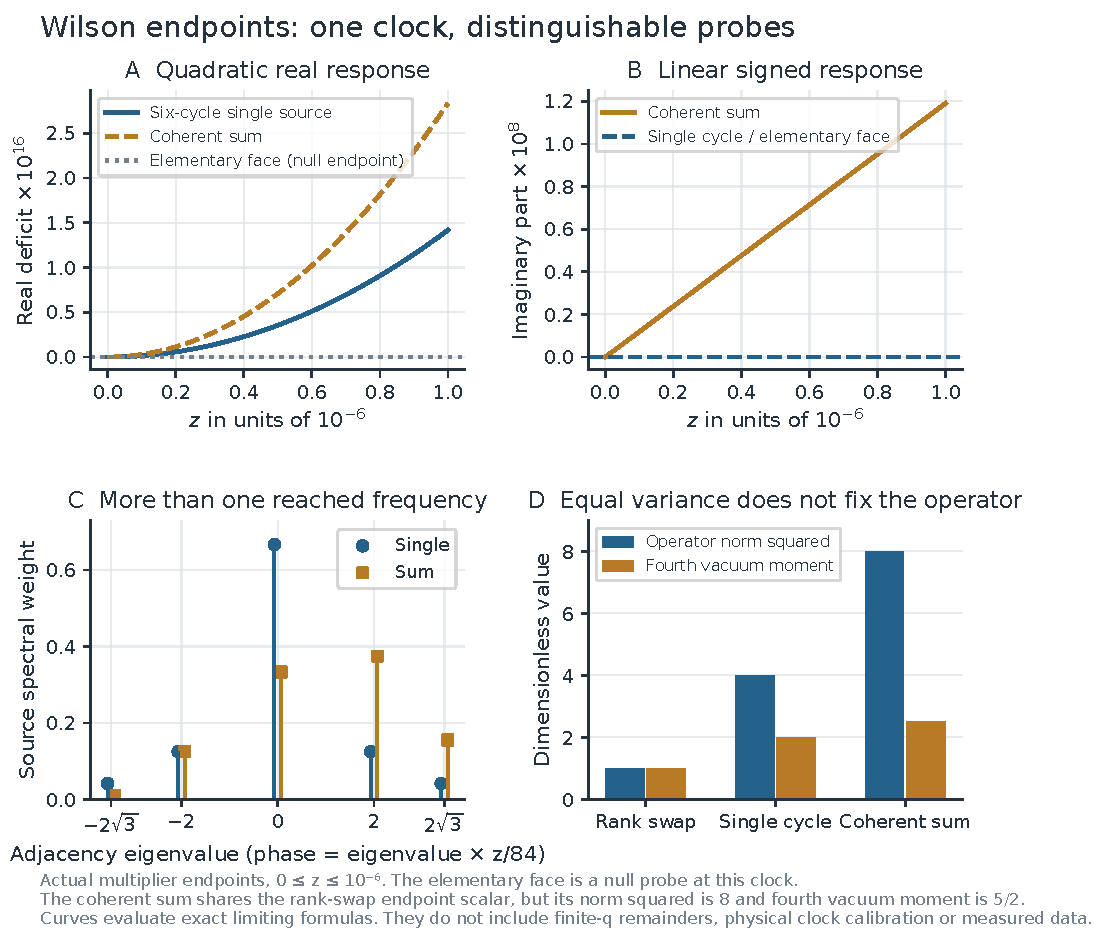
\includegraphics[width=\textwidth]{figures/wilson_endpoints.pdf}
\caption{Canonical endpoint functions for the specified actual Wilson observables, their reached spectral weights, and distinctions between operator norms and moments. The elementary probe supplies a null slow-response control. These are model readouts; finite-$q$ deviations and physical resource costs require their separate bounds.}
\label{fig:wilson-endpoints}
\end{figure}

\begin{figure}[htbp]\centering
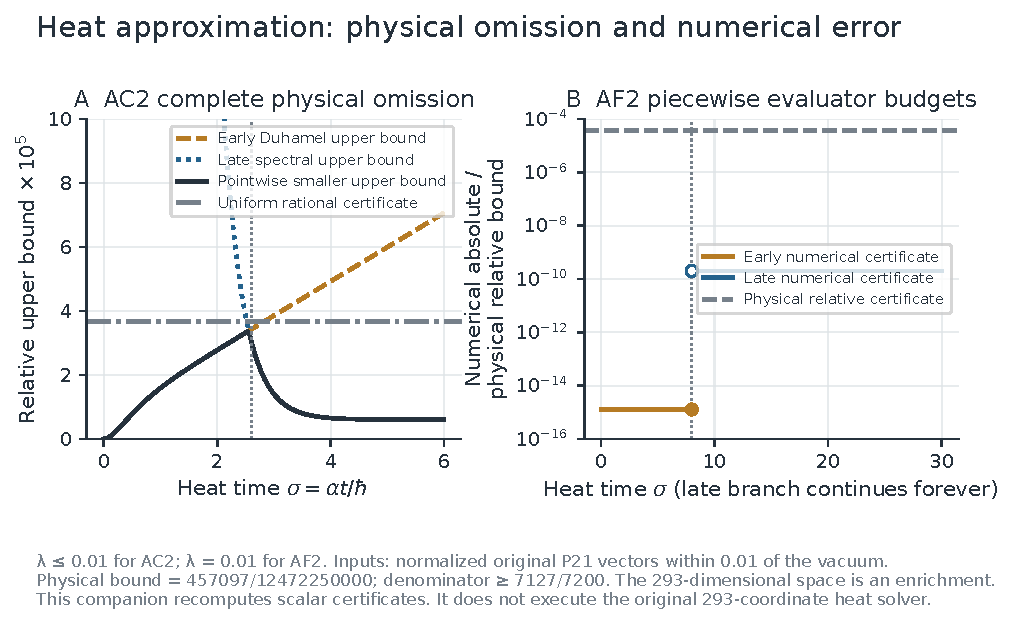
\includegraphics[width=\textwidth]{figures/heat_certificates.pdf}
\caption{The physical AC2 early/late envelope and the separately charged AF2 numerical bound. The numerical branch changes at $\sigma=8$ to prevent secular center error. The denominator applies to the original normalized $P_{21}$ preparation ball; no relative claim for arbitrary ground-null inputs is shown. The late branch extends to all later times even though the horizontal display ends.}
\label{fig:heat-certificates}
\end{figure}
